
\section*{TP 2 : Cercle de Mohr (tenseur des contraintes)}
\begin{itemize}
	\item Représentation de l'état de contrainte en un point considéré
	\item Il faut donc connaître le tenseur de contrainte $\overline{\overline{T}}$
	\item Rappel : $\overline{\overline{T}} = 
	\left(	
	\begin{array}{cc}
	\sigma _x & \tau _{xy} \\ 
	\tau _{xy} & \sigma _y
	\end{array}
	\right) $ est symétrique
\end{itemize}

\subsection*{Conventions}
\noindent \textbf{Attention à l'angle qu'il faut diviser par 2 pour avoir l'équivalent dans le physique.}
\begin{center}
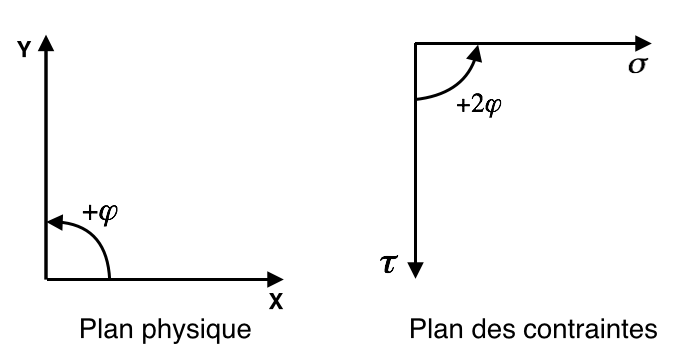
\includegraphics[scale=0.6]{rappels/tp2-1}
\end{center}

\textbf{Dans le plan physique, l'orientation de la facette est celle de $\sigma$ et $\tau$ est perpendiculaire, pointant vers la contrainte de plus grand module !}
\begin{center}
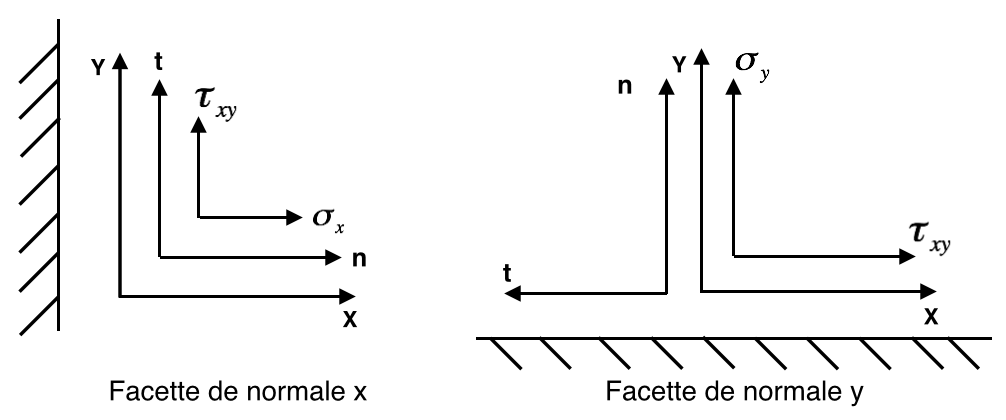
\includegraphics[scale=0.6]{rappels/tp2-2}
\end{center}

\subsection*{Construction}
\begin{equation}
\overline{\overline{T}} = 
	\left(	
	\begin{array}{cc}
	\sigma _x & \tau _{xy} \\ 
	\tau _{xy} & \sigma _y
	\end{array}
	\right) \mbox{ est connu }
\end{equation}
Les composants de la matrice sont les composants du tenseur dans le cercle de Mohr. De cette manière, \textit{x} est représentatif de la facette de normale \textit{x} et \textit{y} pour la facette de normale \textit{y}. On a

\begin{equation}
x(\sigma _x , \tau _{xy}) \qquad y(\sigma _y, - \tau _{xy})
\end{equation}

\begin{itemize}
	\item Valeurs principales : $\sigma _1$ et $\sigma _2$
	\item Directions principales : angle entre l'horizontale et x
	\item Valeurs extrémales : $\tau _{max}$ et $\tau _{min}$
\end{itemize}